% !TEX TS-program = pdflatex
% !TEX encoding = UTF-8 Unicode

% This is a simple template for a LaTeX document using the "article" class.
% See "book", "report", "letter" for other types of document.

\documentclass[11pt]{article} % use larger type; default would be 10pt.
\setcounter{secnumdepth}{2}

\usepackage{paralist} % very flexible & customisable lists (eg. enumerate/itemize, etc.)

\usepackage[utf8]{inputenc} % set input encoding (not needed with XeLaTeX)
\usepackage{float} % to place float images correctly
\usepackage{color} % to color text
\usepackage{enumitem} % for lists
\usepackage{subfigure} % for mockups
\usepackage[font={it}]{caption} % for captions

%%% Examples of Article customizations
% These packages are optional, depending whether you want the features they provide.
% See the LaTeX Companion or other references for full information.

%%% PAGE DIMENSIONS
\usepackage{geometry} % to change the page dimensions
\geometry{a4paper} % or letterpaper (US) or a5paper or....
% \geometry{margin=2in} % for example, change the margins to 2 inches all round
% \geometry{landscape} % set up the page for landscape
%   read geometry.pdf for detailed page layout information

\usepackage{graphicx} % support the \includegraphics command and options

% \usepackage[parfill]{parskip} % Activate to begin paragraphs with an empty line rather than an indent

\usepackage{listings}
\usepackage{color}
 
\definecolor{codegreen}{rgb}{0,0.4,0}
\definecolor{codegray}{rgb}{0.5,0.5,0.5}
\definecolor{codepurple}{rgb}{0.58,0,0.82}
 
\lstdefinestyle{mystyle}{ 
    commentstyle=\color{magenta},
    keywordstyle=\color{blue}\bfseries,
    numberstyle=\tiny\color{codegray},
    stringstyle=\color{codepurple},
    basicstyle=\footnotesize,
    breakatwhitespace=false,         
    breaklines=true,                 
    captionpos=b,                    
    keepspaces=true,                 
    numbers=left,                    
    numbersep=5pt,                  
    showspaces=false,                
    showstringspaces=false,
    showtabs=false,                  
    tabsize=2,
   emph={self}, 
   emphstyle=\color{blue}, 
   emph={[2] BookingManager, FineManager}, 
   emphstyle=[2]\color{codegreen}\bfseries, 
   emph={[3]__init__, newBook, removeReservation, getReservation, manageExpired, min_heap, pop, now, timedelta, expireReservation}, 
   emphstyle=[3]\color{codegreen}, 
}
 
\lstset{style=mystyle}





%%% PACKAGES
\usepackage{booktabs} % for much better looking tables
\usepackage{array} % for better arrays (eg matrices) in maths
%\usepackage{paralist} % very flexible & customisable lists (eg. enumerate/itemize, etc.)
\usepackage{verbatim} % adds environment for commenting out blocks of text & for better verbatim
\usepackage{subfig} % make it possible to include more than one captioned figure/table in a single float
% These packages are all incorporated in the memoir class to one degree or another...

%%% HEADERS & FOOTERS
\usepackage{fancyhdr} % This should be set AFTER setting up the page geometry
\pagestyle{fancy} % options: empty , plain , fancy
\renewcommand{\headrulewidth}{0pt} % customise the layout...
\lhead{}\chead{}\rhead{}
\lfoot{}\cfoot{\thepage}\rfoot{}

%%% SECTION TITLE APPEARANCE
\usepackage{sectsty}
\allsectionsfont{\sffamily\mdseries\upshape} % (See the fntguide.pdf for font help)
% (This matches ConTeXt defaults)

%%% ToC (table of contents) APPEARANCE
\usepackage[nottoc,notlof,notlot]{tocbibind} % Put the bibliography in the ToC
\usepackage[titles,subfigure]{tocloft} % Alter the style of the Table of Contents
\renewcommand{\cftsecfont}{\rmfamily\mdseries\upshape}
\renewcommand{\cftsecpagefont}{\rmfamily\mdseries\upshape} % No bold!

\newcommand{\pe}{PowerEnJoy }
\newcommand{\pecomma}{PowerEnJoy, }
\newcommand{\bul}[1]{\indent$\bullet$ #1\\}

\usepackage{listings}
\usepackage{pxfonts}
%%% END Article customizations

%%% The "real" document content comes below...




\title{Design Document}
\author{Simone Mosciatti \& Sara Zanzottera}

\begin{document}
\maketitle
\newpage
\tableofcontents
\newpage


\section{Introduction}

\subsection{Purpose}

This Design Document aims to provide to everyone involved in the actual development of the application specific insights about the structure of \pecomma its acthitecture's details, the desing patterns we chosed to implement, but also some details about its high level components, their interactions and general behavior.

\subsection{Scope}

\pe is a digital management system for car sharing that exclusively employs electric cars to provide its service. The system provides all the functionalities normally provided by a car sharing service: registering to the service, find the location of nearby available cars, reserve cars up to a short amount of time, unlock the chosen car once found, ride it and then park it in a safe area, when it will be automatically locked and the fee paid.

In addition, the system gives bonuses and penalities in term of discounts or overprices depending on the behavior of the user, in order to promote virtuous behaviors.

\pe is therefore a inherently distributed system, based on a central server interactions with many distributed nodes. In detail the system can be divided into four main parts: 

\begin{itemize}[noitemsep]
	\item a public app, used by customers to access the service
	\item a centralized backend that provides the service
	\item the cars' onboard system, that communicates only with the centralized backend
	\item a reserved fronted, used exclusively by the staff members to better organize their job
\end{itemize}
All these four components will be examined in more detail in the subsequent sections of the document.


\subsection{Definitions, Acronyms, Abbreviations}
 \begin{description}
	\item[RASD] Requirements and Specification Document.
	\item[DD] Design Document.
	\item[User] A customer of \pe using the service.
	\item[Staff Operator] An employee of \pe which takes care of the cars.
	\item[Ride] The action of getting onboard of a \pe car, start its engine, drive to destination and park.
  	\item[Running Time] The time an user spends using the \pe service.
	\item[Issue] Any problem a car may incur in, or a user may face while using the service.
	\item[Nearby Cars] Cars located within a maximum distance to a specific position.
	\item[Nearby Issues] Issues that are affecting cars close to a specific position.
	\item[Booking (Reservation)] The act to reserve a car for a limited amount of time for future use by a user.
	\item[Reservation's maximum time] The maximun amount of time a car can be reserved.
	\item[Driver] Whoever is driving a regularly booked \pe car.
	\item[Passenger] Whoever is in inside a \pe car but is not the driver.
	\item[Driving License] The state's issued driving license of the user.
	\item[Notification] A form of comunication where the user is actively notified of some event.
	\item[Issue Report] An incoming notification that states a car incurred in an issue.
	\item[Fine] A fine issued by the local law enforcing officers to a user while driving a \pe car. 
	\item[Pending Bills] Bills that an user still need to pay to \pe.
	\item[Safe Area] An parking area, predefined by the company, where is possible to safely park the cars of the \pe fleet.
	\item[Battery Charge] The amount of charge that is kept inside the car's battery.
	\item[Charging Station] Dedicated areas where is possible to plug the \pe cars to charge their batteries.
	\item[Car's Onboard System] The controll system of the car that is able to exchange data with the central system and to relevate operation parameters.
	\item[Customer's App] An implementation of the system frontend tailored to the need of the customers.
	\item[Operator's App] An implementation of the system frontend tailored to the need of the staff.
	\item[Central System] The central system for \pe. All the command and all the data are streamed, analyzed and used here.
	\item[Credentials] Pair \{Username, Password\} necessary to access the \pe system.
  	\item[GPS]: Global Positioning System is a global navigation satellite system (GNSS) that provides location and time information in all weather conditions, anywhere on or near the Earth where there is an unobstructed line of sight to four or more GPS satellites.
  	\item[System's Frontend] The interface provided to the user of the \pe system. 
  	\item[System's Backend]  The whole technical infrastructure necessary to \pe.
  \end{description}

\subsection{Document Structure}

\begin{enumerate}
	\item \textbf{Introduction}

	This sections aims to explain the purpose and the scope of the document, introducing the reader to subsequent sections of the document itself.

	\item \textbf{Architectural Design}
	 
	This sections will explain the main architectural decision we made.

	\item \textbf{Algorithm Design}

	In this section we focus on the most critical code section and we provide an in-depth analysis of how they should be structured, eventually providing pseudocode for them.
	
	\item \textbf{User Interface Design}

	In this section we carry on the UX design with the help of UX and BCE diagrams, eventually completing them with updated and extended application mockups.

	\item \textbf{Requirements Traceability}
	
	In this section we map the requirements stated in the RASD to the actual component or processes that fulfill these requirements.

	\item \textbf{Conclusions}

	In this section we enumerate the tools we used to redact this document, the hours of work spent by each group member and the (eventual) revision history of the document itself.
\end{enumerate}

\subsection{Reference Documents}
\begin{itemize}
	\item \textit{Assignments AA 2016-2017.pdf} (Assignments document given by the teacher)
	\item \textit{Sample Design Deliverable Discussed on Nov. 2.pdf} (Sample document provided by the teacher)
  \end{itemize}




\newpage
\section{Architectural Design}
The overall design process has been carried in a bottom-up approach, starting from the analysis of goals and requirements moving upwards to the definition of the higher level components of the system. In the following sections we provide more details on the designed architecture.

\subsection{Design Process Description}

The overall design process starts from the analysis of the goals. 

Taking forward the considerations made in the RASD, we analyse the interface between the world and the machine: given the list of goals and requirements, we identify what interfaces the system need to provide to the users.
If those interfaces would have been alreay implemented our work would have been completed, however such is not the case, and those interfaces require some functionalities.

Once all the necessary functionalities have been identified we organize them into high-level components taking care to respect the ``Single Responsability'' principle in order to provide highly decoupled and reusable components.
Again, if those functionalities were already working our works would have been done, however these components need to be actually implemented and deployed into physical machines.

At this point we proceed to identify the physical nodes of our system and where our components should be deployed in order to fullfil their functionalities. We also analyze what comunication mechanism to use between the node.

Finally we proceed to deploy the components into the physical node.

To double check the correctness of the overall design we produce several sequence diagram showing for the uses cases what functionality is involved and what functionality is called.

The rest of this section follows this flow, starting from the goals analysis and finally providing the overall design.

The next section will show the uses cases.

\subsection{Goals Analysis}

In this part of the document we analyze Goals as defined in RASD, in order to list and describe in detail which interactions betwen the world and the machine will be performed and how to provide them. 

These are named \textbf{SB/FunctionalityName} in order to highlight that these functions are related to the system's boundaries. Indeed we know already that some goals are specific for customers, some are specific for the staff operators, and some are shared. In order to highlight this difference, we decided to enforce the following naming schema:
\begin{itemize}[noitemsep]
	\item SB/ALL/FunctionalityName for shared functionalities
	\item SB/CUST/FunctionalityName for customer's reserved functionalities
	\item SB/STAFF/FunctionalityName for staff's reserved functionalities
\end{itemize}

Many of the following use cases requires some specific funcionalities to be provided by the backend. These are highlighted and named \textbf{Sy/FunctionalityName}, where ``Sy`` indicate an abstract system that we are going to model in detail in the next paragraphs.

\begin{description}
	\item[SB/ALL/Registration] \hfill
	\begin{description}
		\item[Description] Users can register to the system.
		\item[Requires] \hfill
		\begin{itemize}
			\item Sy/Register %$\Leftrightarrow$ USER/Register
			\item Sy/Validate %$\Leftrightarrow$ USER/Validate
		\end{itemize}
	\end{description}
	\item[SB/ALL/Login] \hfill
	\begin{description}
		\item[Description] Users can log into the system providing their email and password and logout from the system.
		\item[Requires] \hfill
		\begin{itemize}
			\item Sy/Login %$\Leftrightarrow$ USER/Login
			\item Sy/Logout
		\end{itemize}
	\end{description}
	\item[SB/CUST/Lookup] \hfill
	\begin{description}
		\item[Description] Users can look for cars near them or near a specific position and range.
		\item[Requires] \hfill
		\begin{itemize}
			\item Sy/GeoLocationCars %$\Leftrightarrow$ GEOLOCATION/AvailableCars
			\item Sy/PositionUser %$\Leftrightarrow$ POSITION/User
		\end{itemize}
	\end{description}
	\item[SB/CUST/Book] \hfill
	\begin{description}
		\item[Description] Users can book cars to use within the next hour.
		\item[Requires] \hfill
		\begin{itemize}
			\item Sy/Book %$\Leftrightarrow$ BOOKING/Book
		\end{itemize}
	\end{description}
	\item[SB/CUST/Unbook] \hfill
	\begin{description}
		\item[Description] Users can remove a previously made reservation.
		\item[Requires] \hfill
		\begin{itemize}
			\item Sy/Unbook %$\Leftrightarrow$ BOOKING/Unbook
		\end{itemize}
	\end{description}
	\item[SB/ALL/Unlock] \hfill
	\begin{description}
		\item[Description] Users can unlock a nearby car that was previously booked.
		\item[Requires] \hfill
		\begin{itemize}
			\item Sy/PositionUser %$\Leftrightarrow$ POSITION/User
			\item Sy/PositionCar %$\Leftrightarrow$ POSITION/Car
			\item Sy/Unlock %$\Leftrightarrow$ CAR/Unlock
		\end{itemize}
	\end{description}
	\item[SB/CUST/Ride] \hfill
	\begin{description}
		\item[Description] Users can ride a reserved car.
		\item[Requires] \hfill
		\begin{itemize}
			\item Sy/StartRide %$\Leftrightarrow$ RIDE/Start
			\item Sy/EndRide %$\Leftrightarrow$ RIDE/End
			\item Sy/ValidateLicense %$\Leftrightarrow$ CAR/ValidateLicense
			\item Sy/GeoLocationAreas %$\Leftrightarrow$ GEOLOCATION/Areas
			\item Sy/Lock %$\Leftrightarrow$ CAR/Lock
		\end{itemize}
	\end{description}
	\item[SB/ALL/SafeAreas] \hfill
	\begin{description}
		\item[Description] Users can locate safe parking areas while driving.
		\item[Requires] \hfill
		\begin{itemize}
			\item Sy/GeoLocationAreas %$\Leftrightarrow$ GEOLOCATION/Areas
		\end{itemize}
	\end{description}
	\item[SB/CUST/UnsafeParking] \hfill
	\begin{description}
		\item[Description] The system reacts to unsafe parking. It first tells users they are going to be fined if they leave the car unsafely parked, then it fines users who leaves the car in an unsafe area.
		\item[Requires] \hfill
		\begin{itemize}
			\item Sy/EngineOff %$\Leftrightarrow$ CAR/TurnOff
			\item Sy/Lock %$\Leftrightarrow$ CAR/Lock
			\item Sy/UnsafeParkNotification %$\Leftrightarrow$  NOTIFY/UnsafePark
			\item Sy/UnsafeParkFine
		\end{itemize}
	\end{description}
	\item[SB/ALL/PowerStation] \hfill
	\begin{description}
		\item[Description] Users can locate and use charging station.
		\item[Requires] \hfill
		\begin{itemize}
			\item Sy/GeoLocationAreas %$\Leftrightarrow$ GEOLOCATION/Areas
			\item Sy/Plugged %$\Leftrightarrow$ CAR/Telemetry
			\item Sy/CarPluggedNotification %$\Leftrightarrow$ NOTIFY/CarPlugged
		\end{itemize}
	\end{description}
	\item[SB/CUST/Charge] \hfill
	\begin{description}
		\item[Description] Users are charged a fee at the end of the ride or if a reservation expires.
		\item[Requires] \hfill
		\begin{itemize}
			\item Sy/SendFee %$\Leftrightarrow$ NOTIFY/SendFee
			\item Sy/BookExpire %$\Leftrightarrow$ BOOKING/Expire
			\item Sy/CalculateUnsafeParkingFee %$\Leftrightarrow$ BILL/Calculate
			\item Sy/CalculateRideFee 
			\item Sy/CalculateExpireBookFee
		\end{itemize}
	\end{description}
	\item[SB/CUST/Payment] \hfill
	\begin{description}
		\item[Description] Users can pay bills through the app and set their default payment method.
		\item[Requires] \hfill
		\begin{itemize}
			\item Sy/MakePayment %$\Leftrightarrow$ BILL/Pay
			\item Sy/SetPaymentMethod %$\Leftrightarrow$ USER/SetPaymentMethod
		\end{itemize}
	\end{description}
	\item[SB/ALL/ReportIssues] \hfill
	\begin{description}
		\item[Description] Users can report issues to the system.
		\item[Requires] \hfill
		\begin{itemize}
			\item Sy/ReportIssue %$\Leftrightarrow$ ISSUE/New
		\end{itemize}
	\end{description}
	\item[SB/STAFF/FindIssues] \hfill
	\begin{description}
		\item[Description] The staff can locate cars that need their intervention.
		\item[Requires] \hfill
		\begin{itemize}
			\item Sy/GeoLocationIssues %$\Leftrightarrow$ GEOLOCATION/Issues
		\end{itemize}
	\end{description}
	\item[SB/STAFF/Support] \hfill
	\begin{description}
		\item[Description] The staff can identify and solve car’s issues.
		\item[Requires] \hfill
		\begin{itemize}
			\item Sy/Lock %$\Leftrightarrow$ CAR/Lock
			\item Sy/Unlock %$\Leftrightarrow$ CAR/Unlock
			\item Sy/TakeChargeIssue  %$\Leftrightarrow$ ISSUE/TakeCharge
			\item Sy/SolveIssue %$\Leftrightarrow$ ISSUE/Solve
			\item Sy/GiveUpIssue %$\Leftrightarrow$ ISSUE/GiveUp
		\end{itemize}
	\end{description}
\end{description}


\begin{figure}[H]
	\centering
	\includegraphics[width=0.6\textwidth]{UML/UI.png}
	\caption{Graphical visulaization of the UI divided by tipology of users.}
\end{figure}	


\subsection{Interfaces Design}

Now we gather all the functionalities we just described and we organize them into higher-level interfaces, being careful at respecting the responsibilities given to each one of them.

In order to clarify how previously defined ``Sy/FunctionalityName`` maps with the interface's specific functions, we used a notation \textbf{INTERFACE/FuncionalityName $\Leftrightarrow$ Sy/FunctionalityName}. The functionality name can vary, according to the context.

\begin{description}
	\item[USER\_MANAGER] \hfill
	\begin{description}
		\item[Responsability] Manages the users.
	\item[USER/Register $\Leftrightarrow$ Sy/Register] \hfill
		\begin{description}[noitemsep]
			\item[Responsability] Registers a new user into the system.
			\item[Input] Information from the user such as:
				\begin{itemize}
					\item First name
					\item Last name
					\item Identity ID
					\item Password
					\item Email
					\item License ID
					\item Credit card informations: credit card number, control code, expiry date, owner, etc.
				\end{itemize}
			\item[Output] The ID of the newly created user.
		\end{description}
	\item[USER/Validate $\Leftrightarrow$ Sy/Validate] \hfill
		\begin{description}[noitemsep]
			\item[Responsability] Validate the information provided by the user, it makes sure that the user is not already registered into the system, that the License is valid as well the credit card information.
			\item[Input] Information from the user such as:
				\begin{itemize}
					\item First name
					\item Last name
					\item Password
					\item Email
					\item License ID
					\item Credit card informations: credit card number, control code, expiry date, owner, etc.
				\end{itemize}
			\item[Output] Confirm correctness and validity of the informations.
		\end{description}
	\item[USER/Login $\Leftrightarrow$ Sy/Login] \hfill
		\begin{description}[noitemsep]
			\item[Responsability] Allows users to log into the system.
			\item[Input] Email (considered a unique user ID) and password.
			\item[Output] A session key, meaning that the user is logged into the system.
		\end{description}
	\item[USER/Logout $\Leftrightarrow$ Sy/Login] \hfill
		\begin{description}[noitemsep]
			\item[Responsability] Allows users to logout the system.
			\item[Input] The login session key.
			\item[Output] The session key is invalidated. 
		\end{description}
	\item[USER/SetPaymentMethod $\Leftrightarrow$ Sy/SetPaymentMethod] \hfill
		\begin{description}[noitemsep]
			\item[Responsability] Update user's information about the preferred payment method.
			\item[Input] The ID of the user and new payment informations.
			\item[Output] The payment method data related to this user is updated.
		\end{description}
	\end{description}
	
	\item[GEOLOCATION] \hfill
	\begin{description}
		\item[Responsability] Locates elements, points and areas of interest around a specific coordinate. ``Search`` service for elements of interest.
	\item[GEOLOCATION/AvailableCars $\Leftrightarrow$ Sy/GeoLocationCars] \hfill
		\begin{description}[noitemsep]
			\item[Responsability] Retrives the position of available cars.
			\item[Input] Search parameters such as:
			\begin{itemize}
				\item Geographical coordinates of the center of the search range (latitude and longitude as provided by GPS sensors) 
				\item Maximum walking distance from the specified position
				\item Other search settings, like minimum battery level, etc.
			\end{itemize}
			\item[Output] A set of available cars matching the search parameters.
		\end{description}

	\item[GEOLOCATION/Areas $\Leftrightarrow$ Sy/GeoLocationAreas] \hfill
		\begin{description} [noitemsep]
			\item[Responsability] Retrives the position of areas of interest, such as power stations and safe parking areas.
			\item[Input] Geographical coordinates of the center of the search range (latitude and longitude as provided by GPS sensors) and a search radius.
			\item[Output] A set of areas of interest inside the circle of radius provided centered on the coordinates provided.
		\end{description}

	\item[GEOLOCATION/Issues $\Leftrightarrow$ Sy/GeoLocationIssues] \hfill
		\begin{description}[noitemsep]
			\item[Responsability] Retrives the position of cars with some issues.
			\item[Input] Search parameters such as:
			\begin{itemize}
				\item Geographical coordinates of the center of the search range (latitude and longitude as provided by GPS sensors) 
				\item Radius of the search
				\item Issue type, Exeption status, and other similar search settings.
			\end{itemize}
			\item[Output] A set of cars with issues matching the search parameters inside the circle of radius provided centered on the coordinates provided.
		\end{description}
		
	\item[GEOLOCATION/IsSafeArea $\Leftrightarrow$ Sy/GeoLocationIssues] \hfill
		\begin{description}[noitemsep]
			\item[Responsability] Given the coordinates check if those coordinates are inside a safe area.
			\item[Input] Coordinates.
			\item[Output] A boolean indicating if the coordinates are inside a safe area.
		\end{description}
		
	\end{description}

	\item[POSITION] \hfill
	\begin{description}
		\item[Responsability] Locates elements of interest given their ID. ``Lookup`` service for elements of interest.
	\item[POSITION/Car $\Leftrightarrow$ Sy/PositionCar] \hfill
		\begin{description}[noitemsep]
			\item[Responsability] Retrieves the position of a specific car.
			\item[Input] The ID of the car.
			\item[Output] The coordinates of the car.
		\end{description}
	\item[POSITION/User $\Leftrightarrow$ Sy/PositionUser] \hfill
		\begin{description}[noitemsep]
			\item[Responsability] Retrieves the position of an user.
			\item[Input] The ID of the user.
			\item[Output] The coordinates of the user.
		\end{description}
	\item[POSITION/Areas] \hfill
		\begin{description}[noitemsep]
			\item[Responsability]Retrieves the position of an area of interest.
			\item[Input] The ID of the area.
			\item[Output] The coordinates of the area as a set of boundary points.
		\end{description}
	\end{description}
	
	\item[BOOKING\_MANAGER] \hfill
	\begin{description}
		\item[Responsability] Manages reservations.
	\item[BOOKING/Book $\Leftrightarrow$ Sy/Book] \hfill
		\begin{description}[noitemsep]
			\item[Responsability] Books one available car.
			\item[Input] The ID of the car and the ID of the user.
			\item[Output] The car is booked and the ID of the reservation is provided.
		\end{description}
	\item[BOOKING/Unbook $\Leftrightarrow$ Sy/Unbook] \hfill
		\begin{description}[noitemsep]
			\item[Responsability] Removes a reservation.
			\item[Input] The ID of the user and the ID of the reservation.
			\item[Output] The reservation is cancelled.
		\end{description}
	\item[BOOKING/Expire $\Leftrightarrow$ Sy/BookExpire] \hfill
		\begin{description}[noitemsep]
			\item[Responsability] Removes an expired reservation and fines the related user.
			\item[Input] ID of the reservation.
			\item[Output] The reservation is cancelled and the user is fined.
		\end{description}	
	\end{description}
	
	\item[CAR\_MANAGER] \hfill
	\begin{description}
		\item[Responsability] Manages the iteractions between users and cars.
	\item[CAR/Unlock $\Leftrightarrow$ Sy/Unlock] \hfill
		\begin{description}[noitemsep]
			\item[Responsability] Unlocks the car.
			\item[Input] The ID of the car and the ID of the user asking to unlock.
			\item[Output] The car is unlocked.
		\end{description}
	\item[CAR/ValidateLicense $\Leftrightarrow$ Sy/ValidateLicense] \hfill
		\begin{description}[noitemsep]
			\item[Responsability] Confirms the scanned license is related to the user who booked the car.
			\item[Input] The scanned image of the driving license and the ID of the booking
			\item[Output] The car is unlocked.
		\end{description}
	\item[CAR/Lock $\Leftrightarrow$ Sy/Lock] \hfill
		\begin{description}[noitemsep]
			\item[Responsability] Locks the car.
			\item[Input] The ID of the car.
			\item[Output] The car is locked.
		\end{description}
	\item[CAR/TurnOff $\Leftrightarrow$ Sy/EngineOff] \hfill
		\begin{description}[noitemsep]
			\item[Responsability] Turns off the engine of a car.
			\item[Input] The ID of the car.
			\item[
Output] The car is turned off.
		\end{description}
	\item[CAR/Telemetry] \hfill
		\begin{description}[noitemsep]
			\item[Responsability] Retrieves real-time, updated informations about a car.
			\item[Input] The ID of the car.
			\item[Output] All the latest informations available about the car.
		\end{description}
	\item[CAR/SetStatus] \hfill
		\begin{description}[noitemsep]
			\item[Responsability] Sets the Exception status of a car to a new value.
			\item[Input] The ID of the car and the new status.
			\item[Output] The new status is set.
		\end{description}
	\item[CAR/GetDetails] \hfill
		\begin{description}[noitemsep]
			\item[Responsability] Returns all available data about a given car (such as battery level, charging status, etc.).
			\item[Input] The ID of the car.
			\item[Output] All available details about the car
		\end{description}
	\end{description}
	
	\item[RIDE\_MANAGER] \hfill
	\begin{description}
		\item[Responsability] Manage the rides.
	\item[RIDE/Start $\Leftrightarrow$ Sy/StartRide]  \hfil
		\begin{description}[noitemsep]
			\item[Responsability] Start counting the time of the ride.
			\item[Input] The ID of the user and the ID of the booking.
			\item[Output] The ID of the ride.
		\end{description}
	\item[RIDE/End $\Leftrightarrow$ Sy/EndRide] \hfil
		\begin{description}[noitemsep]
			\item[Responsability] Stop counting the time of the ride.
			\item[Input] The ID of the ride.
			\item[Output] Stop the count of time for the ride.
		\end{description}
	\item[RIDE/FindRides] \hfill
		\begin{description}[noitemsep]
			\item[Responsability] Retrieve the list of rides done with a specific car in a defined time range.
			\item[Input] The ID of the car and a time range.
			\item[Output] The list of rides performed with that car in that time range.
		\end{description}
	\end{description}
	
	\item[BILLING\_MANAGER] \hfill

	\begin{description}
		\item[Responsability] Manages all the fees.
	\item[BILL/CalculateRideFee $\Leftrightarrow$ Sy/CalculateRideFee] \hfill
		\begin{description}[noitemsep]
			\item[Responsability] Calculates the amount of a riding fee.
			\item[Input] The ID of the ride.
			\item[Output] The ID of the fee with a complete total which include eventual discounts or overprices.
		\end{description}
	\item[BILL/CalculateExpireBookFee $\Leftrightarrow$ Sy/CalculateExipreBookFee ] \hfill
		\begin{description}[noitemsep]
			\item[Responsability] Calculates the amount of a expired prenotation fee.
			\item[Input] The ID of the booking.
			\item[Output] The ID of the fee refered to the expired prenotation.
		\end{description}
	\item[BILL/CalculateUnsafeParkingFine $\Leftrightarrow$ Sy/CalculateUnsafeParkingFee] \hfill
		\begin{description}[noitemsep]
			\item[Responsability] Requires user to pay a fine for an unsafe parking.
			\item[Input] The ID of the ride which left the car unsafely parked.
			\item[Output] The ID of the fee refered to the fine for unsafe parking.
		\end{description}
	\item[BILL/Pay $\Leftrightarrow$ Sy/MakePayment] \hfill
		\begin{description}[noitemsep]
			\item[Responsability] Requires user to pay a specific fee.
			\item[Input] The ID of the user and the ID of a fee.
			\item[Output] The fee is paid.
		\end{description}
	\end{description}

	\item[ISSUE\_MANAGER] \hfill
	\begin{description}
		\item[Responsability] Manages car's issues.
	\item[ISSUE/New $\Leftrightarrow$ Sy/ReportIssue] \hfill
		\begin{description}[noitemsep]
			\item[Responsability] Rise a new issue.
			\item[Input] ID of the car, ID of the user raising the issue, a title and a description of the issue.
			\item[Output] The ID of the reported issue.
		\end{description}
	\item[ISSUE/TakeCharge $\Leftrightarrow$ Sy/TakeChargeIssue] \hfill
		\begin{description}[noitemsep]
			\item[Responsability] Allows operators taking in charge of a particular issue.
			\item[Input] The ID of the issue, the ID of the operator.
			\item[Output] The operator is now responsable for the issue.
		\end{description}
	\item[ISSUE/Solve $\Leftrightarrow$ Sy/SolveIssue] \hfill
		\begin{description}[noitemsep]
			\item[Responsability] Allows operators to close an issue marking it as Solved. The system is resposible of allowing this operation only if it can confirm the issue has been solved.
			\item[Input] The ID of the issue, the ID of the operator.
			\item[Output] The issue is set as Solved, or set as Closed and another new issue is opened.
		\end{description}
	\item[ISSUE/GiveUp $\Leftrightarrow$ Sy/GiveUpIssue] \hfill
		\begin{description}[noitemsep]
			\item[Responsability] Allows operators to give up over an issue.
			\item[Input] The ID of the issue, the ID of the operator.
			\item[Output] The issue is no more related to the specified operator and available for others to be took in charge.
		\end{description}
	\end{description}
	
	\item[NOTIFIER] \hfill
	\begin{description}
		\item[Responsability] This component takes care to notify user of events.
	\item[NOTIFY/Notify $\Leftrightarrow$ \{Sy/SendFee, Sy/UnsafeParkNotification, Sy/CarPluggedNotification\}] \hfill
	\begin{description}[noitemsep]
			\item[Responsability] Notify the user of some event, it may also prompt the user to acknoledge some fact or complete some action.
			\item[Input] A notification object.
			\item[Output] The notification is show to the user and the user may be prompted to do some action.
		\end{description}
	\end{description}
\end{description}


{\color{blue} { Qui un Components View simile a quello a pagina 8 dell'esempio... possibilmente con un font un po' piu' grande che nell'esempio. \\ Non so bene se qui o in fondo alla sezione successiva. }}
\\

In this part of the design we made some choices where alternative approach may have been considered as well. We now motivate some of those choices.

\subsubsection{Notifier}

To make the user able to receive notification from server we could use several strategies. In a static world, where the product doesn't change, all of the choice are equivalent. However, if we put ourselves in a dynamic situation where the goals and requirements of the software evolve, our choice are more critical and must be justified.

Before deciding for an isolated component responsible only to forward a notification to the user, we evaluated other options for the notifier:

\begin{enumerate}
	\item Each component could have its own NOTIFIER: eg. instead of NOTIFY/Notify(Notification) we could have something like CAR/NotifyUnsafePark(). Indeed, as more components need to notify the user, more and more different versions of the same functionality will probably be reimplemented in different part of the code base: a problem we would like to avoid.
	\item Each kind of notification could have its own function: eg. instead of NOTIFY/Notify(Notification) we could have something like NOTIFY/UnsafePark(). We believe this choice would make the overall developing time too slow, since every new functionality which requires a notification would have to be implemented into NOTIFY, making it unstable.
\end{enumerate}

We believe that our choice allows a very fast development cycles while maintaining an high decoupling between different components.




\subsection{Communication Design}

Once we have identified the abstract interfaces that, together, provide the functionalities of our system, we are going to design the components which implements them.

In order to actually implements the components we first need to know where those components are deployed, and the form of comunication used between or inside them.

\subsubsection{Physical structure}

As for the RASD (section 2: Overall Description), the system is be divided into four parts:
\begin{itemize}[noitemsep]
	\item the \textbf{customer's app}, used by customers to access the service.
	\item the \textbf{staff's app}, used exclusively by the staff members to better organize their job.
	\item the \textbf{main server}, a centralized backend that provides the service.
	\item the \textbf{cars’ onboard system}, that communicates only with the centralized backend.
\end{itemize}

As said in the RASD, also in this Design Document we are using the term ``App`` to refer to a User Interface deployed on a smartphone, and we will keep such terminology for sake of clarity. However it must be clear that a whole spectrum of technologies could be used to actually implement the user Interface, not only mobile application.

Also, for the scope of this analysis we often consider the customer's app and the staff's app as a single entity, called simply ``app''.

At a first glance, the above elements can be organized in a two-tier Client-Server architecture as follows:
\begin{itemize}[noitemsep]
	\item Tier 1, the main server, which handles Application Logic and Data Management.
	\item Tier 2, comprising mobile apps and cars, hosts the User Interface.
\end{itemize}
From now on, we design the system basing on these fundamentals elements, defining their roles and interactions.


\end{description}
\begin{figure}[H]
	\centering
	\includegraphics[width=0.6\textwidth]{UML/HighLevelComponents.png}
	\caption{Higher level components of the system}
\end{figure}	


\subsubsection{Communication Strategy}

Now that our nodes are defined, we need to design the comunication protocols between them.

It would have been possible to make each node comunicate with each other node: however this approach raises some concerns about the security of the system, especially for the communication between the users and the cars (see below). 

Of course a well done, and a well tested system should not raise these concerns, however real word engineering is constrained and the authors believe that a more defensive and conservative approach is more suitable.

Following these consideration we decided that would be more maneagable to have only two communication channels:
\begin{itemize}[noitemsep]
	\item one between the main server and the user apps;
	\item another one between the main server and the cars.
\end{itemize}

We decide to completely avoid all kinds of communication between the cars and the apps. 

The main server always acts as an intermediary for app-to-car and car-to-app communications, in order for the system to have full control on these otherwhise completely hidden interactions.

\subsubsection{Interactions with 3rd-parties}
We decided to prevent any access to third-part services to every component but the main server, mainly for security reasons.

The main server will expose the necessary APIs to apps and cars to allow them retrieving all the informations they need without having them communicating indipendently with any external service.

\subsubsection{Communication Protocols}

The communication between the main server and the user will employ a simple \textbf{Client-Server} approach which seems to naturally fit the domain space, it is a well know industry standard and is widely used.

On the other hand, communications between the server and the fleet is clearly more suitable for a \textbf{Publisher-Subscriber} pattern. The car has to communicate very often a lot of valuable information to the main server, and a PubSub pattern achieves high troughput and low latency. Even if the Pub-Sub pattern may not be so widely used and know, our experience suggested that the trade-off is well worth.

Moreover, we decided to model the most part of external services as Web services, so the server will communicate with them using a \textbf{Service-Oriented} approach.


\begin{figure}[H]
	\centering
	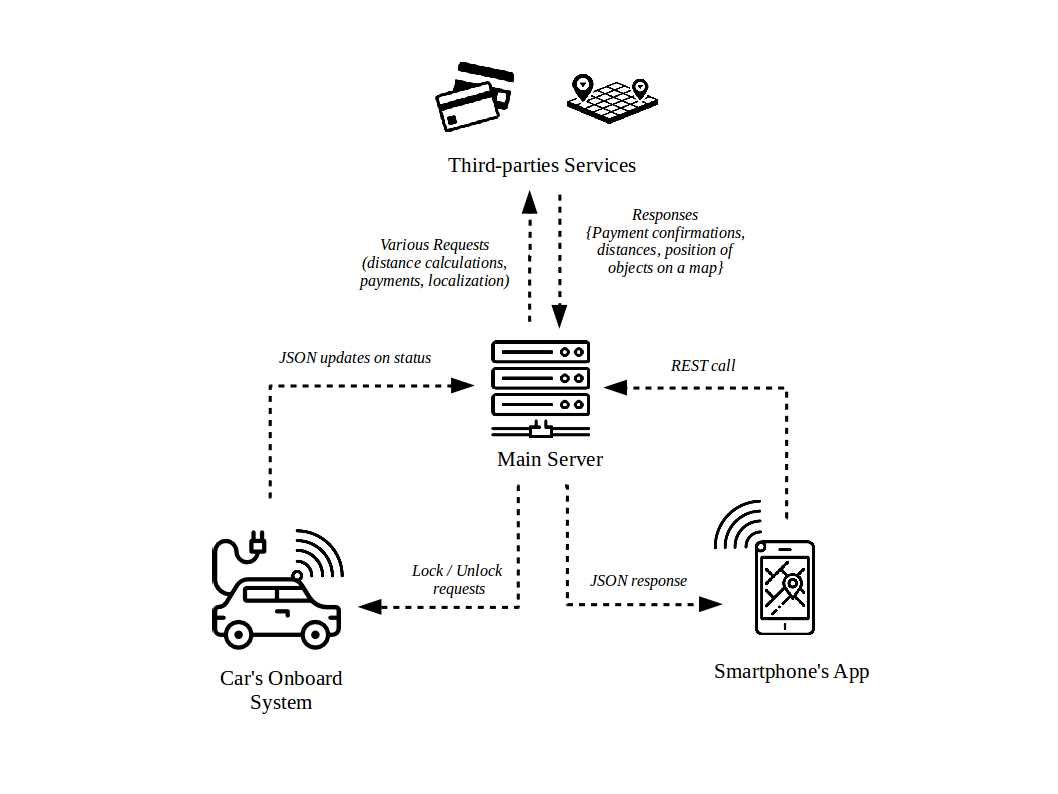
\includegraphics[width=1\textwidth]{proposed_system.png}
	\caption{Communication design of the process (anticipating some technology choices we are going to justify in next sections).}
\end{figure}







\subsection{Components Design}

Up to this point we defined the logical components of the system in terms of interfaces and communication protocols. We now proceed deploying them on the physical nodes identified above in order to end up with a complete, high-level logical architecture for our system.

\begin{description}
	\item[USER\_MANAGER] \hfill \\
	Considering that all its functionalities are exposed as API by the server to the apps, the component is deployed on the server entirely.
		
	\item[GEOLOCATION] \hfill \\
	Considering that all its functionalities are exposed as API by the server, the component is deployed on the server entirely.

	\item[POSITION] \hfill \\
	This component need the partecipation of both users and cars. Thus the component is deployed on all the three nodes:  user apps, cars and the main server.
	\begin{description}
		\item[POSITION/Users] is deployed as \textbf{USER\_POSITION} on the user apps.
		\item[POSITION/Cars] is deployed as \textbf{CAR\_POSITION} on the cars.
		\item[POSITION/Areas] is deployed as \textbf{COORDINATOR} on the main server, as it acts as a dispatcher for all incomig requests, keeps a cache of the retrieved data, and so on.
	\end{description}
	
	\item[BOOKING\_MANAGER] \hfill \\
	Considering that all its functionalities are exposed as API by the server, the component is deployed on the server entirely.
	
	\item[CAR\_MANAGER] \hfill \\
	This component requires a deeper analysis, as its interfaces are exposed by different elements. In details:
	\begin{itemize}
		\item CAR/Unlock is exposed by Server to Apps
		\item CAR/GetDetails is exposed by Cars to Server
		\item CAR/ValidateLicense is exposed by Server to Cars
		\item CAR/Lock is exposed by Cars to Server
		\item CAR/TurnOff is exposed by Cars to Server
		\item CAR/Telemetry is exposed by Cars to Server
		\item CAR/SetStatus is exposed by Cars to Server
	\end{itemize}
\end{description}
	
Thus we create two CAR\_MANAGER subcomponents:
	\begin{description}
		\item[REMOTE\_CAR\_MANAGER] \hfill \\ Comprises all the functions exposed by the server:
		\begin{itemize}
			\item CAR/Unlock
			\item CAR/GetDetails
			\item CAR/ValidateLicense
		\end{itemize}
		\item[LOCAL\_CAR\_MANAGER] \hfill \\ Comprises all the functions exposed by the cars:
		\begin{itemize}
			\item CAR/Lock
			\item CAR/TurnOff
			\item CAR/Telemetry
			\item CAR/SetStatus
		\end{itemize}
	%\end{description}

	\item[RIDE\_MANAGER] \hfill \\
	Considering that all its functionalities are exposed as API by the server to the customer's apps, the component is deployed on the server entirely.

	\item[BILLING\_SYSTEM] \hfill \\
	Considering that all its functionalities are exposed as API by the server to the customer's apps, the component is deployed on the server entirely. 

	\item[ISSUE\_MANAGER] \hfill \\
	Considering that all its functionalities are exposed as API by the server to the customer's apps, the component is deployed on the server entirely. \\
	Indeed, ISSUE/Solve involves an interface that is exposed by the car: thus we define another subcomponent, \textbf{VALIDATE\_SOLVE}, to be deployed on the car to fulfill this function.

	\item[NOTIFIER] \hfill \\
	Considering that its functionality is exposed by the user app, this component is deployed entirely on the user app.

\begin{figure}[H]
	\centering
	\includegraphics[width=0.88\textwidth]{UML/Deploy.png}
	\caption{Graphical visualization of the abstract components needed.}
\end{figure}	

\begin{figure}[H]
	\centering
	\includegraphics[width=1.1\textwidth]{UML/InterfaceDiagram.png}
	\caption{Diagram od the interfaces identified above.}
\end{figure}	





\subsection{Runtime View}

\subsubsection{Register and Login}
\begin{figure}[H]
	\centering
	\includegraphics[width=1\textwidth]{UML/DDSequenceDiagramLoginReg.png}
	\caption{Sequence Diagram for Registration and Login process of customers.	}
\end{figure}	
Here we can clearly see how the responsibility of managing users is set to the \textbf{User\_Manager} component, fully deployed on the main server.

PublicAppGUI is simply responsible of gathering useful data and sending it to User\_Manager, which takes care of contacting external services if needed. 

When the registration/login process is completed server-side, User\_Manager returns control to PublicAppGUI, that is in charge of informing the user about the result of their request and eventually redirected to another page (login after registration is completed successfully, homepage after login is completed successfully).

\subsubsection{Lookup and Book}
\begin{figure}[H]
	\centering
	\includegraphics[width=1\textwidth]{UML/DDSequenceDiagramBooking.png}
	\caption{Sequence Diagram for Lookup and Booking process of customers.}
\end{figure}
This diagram shows clearly the two processes of looking for available cars and booking.

The first goals is achieved with the sole need of GeoLocation, deployed only server-side, that hides to the final user the interaction with linf.io, which is an external service. The app is only responsible of rendering the informations into an interactive map the user can easily navigate.

Once on the map, users can navigate cars details without the need to connect anymore with the server (all the required data has been cached from the previous call) until they decide to book a car. At that moment, a call to Booking\_Manager is issued, which handles the full procedure internally.

The app is responsible only to provide the user feedback about the successfullness of the operation once Booking\_Manager returns.

Note that, after a booking is completed successfully, the user is redirected to the Bookings Page, because it is not possible for a user to issue multiple reservations at the same time.


\subsubsection{Ride}
\begin{figure}[H]
	\centering
	\includegraphics[width=1\textwidth]{UML/DDSequenceDiagramRide.png}
	\caption{Sequence Diagram for the Riding process of customers.}
\end{figure}

This diagram describes what's probably the most complex interaction between users, cars and the main server.

The first step, unlocking the car, is straightforward: Car\_Manager receives a call fro PublicAppGUI requiring the unlock, and Car\_Manager handles internally the process. Notice that, as Car\_Manager is deployed both on the car and on the main server, the call to Car\_Manager/unlock( IDUser, IDCar ) hides another internal process where the server communicates with the car.

Then the driver has to scan its driving licence in order to unlock the engine of the car. Again, Car\_Manager handles some communication between the car's system and the server internally, validate the licence and, if everything is fine, unlocks the engine (step not shown, as it is considered an internal call).

Once the engine is switched on, or 5 minutes from unlocking has passed (regardless of the engine status), Car\_Manager calls Ride\_Manager and starts a new Ride. The lenght of the ride is calculated from this moment until the Ride is closed (see later).

During the whole ride, CarGUI receives continuous updates from Car\_Manager about nearby safe areas and charging station: this data has been retrieved from GeoLocation, that in turn obtained them with a call to linf.io.

When the user exits from the car (regardless of the engine status), Car\_Manager reacts checking if the car has been left in a safe area or not calling GeoLocation/CheckIntoSafeArea( location ).

If not, a series of operations are performed. First, a notification is sent to CarGUI in order to notify the user and possibly have them back in the car. If the user does not come back within a short amount of time (a minute, for example), the engine is switched off, the car is locked, its Exception status is set to ``Unsafely parked`` and a fine is sent to the driver's app.

Otherwhise, the system waits for the car to get locked. Once the locking requests arrives, first the ride is ended with a call to Ride\_Manager/endRide( IDRide ) and the car is locked. Then the regular fee is calculated and the payment issued.


\subsubsection{Issue Management}
\begin{figure}[H]
	\centering
	\includegraphics[width=0.9
\textwidth]{UML/DDSequenceDiagramIssue.png}
	\caption{Sequence Diagram for the Issue Management process for staff operators.}
\end{figure}

In the above diagram we can see how the process of managing issues is carried on by staff operators.

The process share more or less the same workflow as the booking and unlock process for customers, plus some steps related specifically to issues.

It is evident how these additional steps are all managed by Issue\_Manager alone, as to highlight the single, coherent responsibility we assigned to components.


\subsection{Deployement View}

In order to better understand the technology we chosed to design this deployment diagram, refer to section 2.8: Selected Technologies

\begin{figure}[H]
	\centering
	\includegraphics[width=0.8\textwidth]{UML/DeployementView.png}
	\caption{Deployement View of the system}
\end{figure}



\subsection{Selected Technologies}

Having defined the interface between the several functionality provided by the components, all possible communication technologies may have been choosen. Obviously some choices are more apt than others with the respect of latency, throughput, elegance of the design and other factors; however the whole design will remain intact whichever technology we choose.

Here we simply give some reasonable suggestions for protocols and technologies that seems us a better fit for the system we modeled.

\subsubsection{RESTful API}

The main server will expose its API in the most conventional way, using the classical HTTP/TCP/IP stack. In particular we provide RESTful interfaces. Model everything as an entity provides enough capabilities to actual implement the whole system while remaining constrainted to only the basic REST verb. This helped a lot in keeping the whole API scheme simple to understand and to implement.

Apps consume the REST interface provide by the server, however to implement the communication between the server and the app we will use the long polling strategy.

\subsubsection{MQTT}

As for now, most of the communication between the server and the car will happens using the PubSub protocol, while some special messages (like, for example, the ValidateSolve function) will stay on a more basic Client-Server approach.

 Between all the implementation of the PubSub protocol we chose to use MQTT for its low overhead, its QoS and because it is widely used in the industry.

\subsubsection{Nginx}

We decided to use Nginx on the main server instead of a more common Apache server. This choice has been made with care, because Apaceh is surely a more widely used standard for running servers, whereas Nginx is a younger, less used solution. 

Indeed, considering our server is going to handle a lot of parallel operations, we chose a software designed exactly to tackle this issue better than standard Apache-based solutions.

{\color{red} {what about this?}}

\subsubsection{Database}

{\color{red} {what about this?}}









\newpage
\section{Algorithm Design}

In this section we define a first sketch of a BOOKING\_MANAGER, clearly this implementation is extremely naive, it doesn't take care of persisting its status nor it doesn't validate the input, however is effective to show our intention and expectation from the implementator.

\hfil\\

\lstinputlisting[language=Python, breaklines=true,]{Algo/BookingManager.py}

\newpage
\section{User Interface Design}

\subsection{Mockups}
Mockups have already been included in the RASD (section 3.3: Non Functional Requirements) 

\subsection{UX Diagrams}

\begin{figure}[H]
	\centering
	\includegraphics[width=0.88\textwidth]{UML/UXDiagramStaffApp.png}
	\caption{UX Diagram of the interface of staff's application}
\end{figure}	

\begin{figure}[H]
	\centering
	\includegraphics[width=0.88\textwidth]{UML/UXDiagramPublicApp.png}
	\caption{UX Diagram of the interface of customer's application}
\end{figure}

\subsection{BCE Diagrams}

\begin{figure}[H]
	\centering
	\includegraphics[width=1\textwidth]{UML/BCEDiagramStaffApp.png}
	\caption{BCE Diagram of the interface of staff's application}
\end{figure}	
	
\begin{figure}[H]
	\centering
	\includegraphics[width=1\textwidth]{UML/BCEDiagramPublicApp.png}
	\caption{BCE Diagram of the interface of customer's application}
\end{figure}	



\newpage
\section{Conclusions}

\subsection{Tools used}
During the development of this document we used the following tools:
\begin{itemize}
	\item \textbf{Github} to version control the project
	\item \textbf{\LaTeX} on TeXworks to redact this document
	\item \textbf{www.draw.io} to draw UML graphs
	\item \textbf{Gimp v.2.8} to mockup the application
	\item \textbf{LibreOffice Draw} to draw the system's overview at section 2.1
\end{itemize}

\subsection{Hours of work}
\begin{itemize}
	\item SZ: 1h on 30/11
	\item SM: 5h on 2/12
	\item SZ: 5h on 2/12
	\item SZ: 3h on 4/12 (RASD review)
	\item SZ: 3h on 5/12
	\item SZ: 4h on 6/12
	\item SZ: 7h on 7/12
	\item SZ: 10h on 9/12 
	\item SZ: 12h on 10/12
\end{itemize}


\end{document}  
